\chapter{LSTMs para clasificación de series temporales}
En este capítulo se describirán el uso de las LSTM para problemas de series temporales de clasificación, así como una pequeña descripción de las LSTM y las series temporales de clasificación.
\section{Descripción}
Las LSTM son un tipo de red recurrente, esto quiere decir que tiene la capacidad de utilizar como entrada información que ya ha sido procesada; en el caso de las LSTM, dicha información es de gran importancia ya que es utilizada para calcular la salida de la LSTM a parte de la nueva información que se haya obtenido.\newline

\begin{figure}[h]
	\centering
	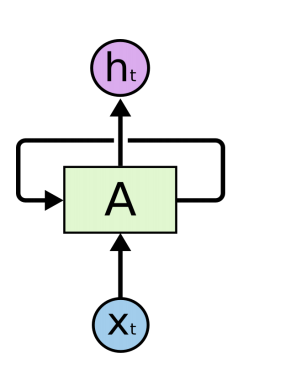
\includegraphics[width=40mm]{imagenes/lstm_basico.png}
	\label{fig:31}
\end{figure}
\verticalspace

Las series temporales de clasificación son un caso especial de serie temporal, ya que el objetivo tras estas series no es obtener una predicción sobre el comportamiento futuro de la serie sino predecir una clase. Sobre este tipo de series temporales se pueden distinguir dos tipos, aquellos donde la serie entera corresponde con una clase y otros donde cada instante de la serie corresponde con una clase. El primer caso se podría expresar de la siguiente forma $ S \rightarrow Y $ donde $S$  es una serie cualquiera e $Y$ es la clase asociada a esta serie. El segundo caso se podría expresar de la siguiente forma $ S = (S_0, S_1,..., S_m) \rightarrow (Y_0,Y_1,..., Y_n) $ donde $S$ es una serie temporal de clasificación de longitud $n$, $S_i$ representa la serie en un momento determinado e $Y_i$ la clase asociada a dicho momento.\newline

\section{Arquitectura}
Para procesar series temporales de clasificación con LSTM se debe utilizar una estructura como la siguiente; una primera capa formadas por LSTM y una segunda capa para la predicción de la clase, esta capa no tiene porque ser LSTM.\newline

La primera capa de esta red es la encargada de procesar la información, las LSTM procesan una serie temporal o un trozo de una serie, dependiendo del tipo de problema que se esté procesando, en cada momento; una vez procesada la información la salida de cada una de las LSTM se pasa a la segunda capa que es la encargada de predecir la clase correspondiente. Para el cálculo de la clase se utiliza una función de activación, para el caso de problemas de clasificación binaria se puede utilizar una función sigmoide, si se trata de un problema de clasificación múltiple se puede añadir tantas neuronas como clases diferentes hay o utilizar la función de activación softmax, que tiene un comportamiento muy parecido a la función sigmoide pero está adaptada a más de dos clases.\newline

Una vez se ha calcula la clase, al igual que cualquier otra red neuronal,  se comprueba si esta es correcta y se recalculan los pesos de las neuronas de la red para mejorar el rendimiento de esta; al tratarse de un problema de clasificación, las métricas de rendimiento deben ser las usuales para clasificación como por ejemplo Accuracy.\newline

La red descrita arriba es un ejemplo de la arquitectura más simple necesaria para afrontar este tipo de problemas. A partir de esta red pueden crearse redes más complejas y que en problemas específicos pueden tener un mejor rendimiento, como por ejemplo añadiendo más capas intermedias o combinando esta red con una red convolucional.\newline
\newpage
Para este trabajo se utilizará la red básica descrita, ya que se utilizarán problemas diferentes para los cuales unas estructuras pueden ser más útiles que otras.

\begin{figure}[h]
	\centering
	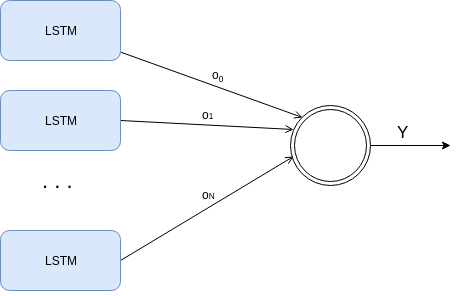
\includegraphics[width=80mm]{imagenes/arquitectura_base.png}
	\label{fig:32}
	\caption{Estructura básica de una red de LSTM para clasificación}
\end{figure}
\verticalspace

\section{Justificación}
Las series temporales son un tipo de dato que tiene dependencia temporal, es decir, el valor de una serie en un momento determinado está relacionado con el valor de la serie en momentos anteriores. Como se ha dicho al principio del capítulo, las LSTM son un tipo de red que utilizan la información anterior para procesar nueva información, por lo que lo hace adecuado para este tipo de problema.\newline

Además, las redes LSTM actualmente son un tipo de red muy utilizada en problemas complejos como la detección del habla, traducción, reconocimiento de palabras escritas a mano o incluso son utilizadas para la creación de IA capaces de jugar a videojuegos mejor que una persona.\newline

A parte de las LSTM, existen otro tipo de neuronas recurrentes como son el caso de las RNN; fueron la primera estructura recurrente para redes neuronales, tienen el inconveniente de no ser capaces de recordar información durante mucho tiempo; o las GRU, son también un tipo de neurona muy utilizada, más sencilla que las LSTM ya que tiene un número de puertas lógicas menor y más adecuada dependiendo del problema, sin embargo, al ser más sencilla no es tiene tanta potencia como las LSTM.\newline

\newpage
Por todo esto, las LSTM son una estructura válida para este trabajo y serán las que se utilicen para procesar los diferentes problemas de clasificación que se verán más adelante.\newline

